\section{\gls{doris} Observation Equation}\label{sec:doris-observation-equation}

\begin{figure}
  \centering
  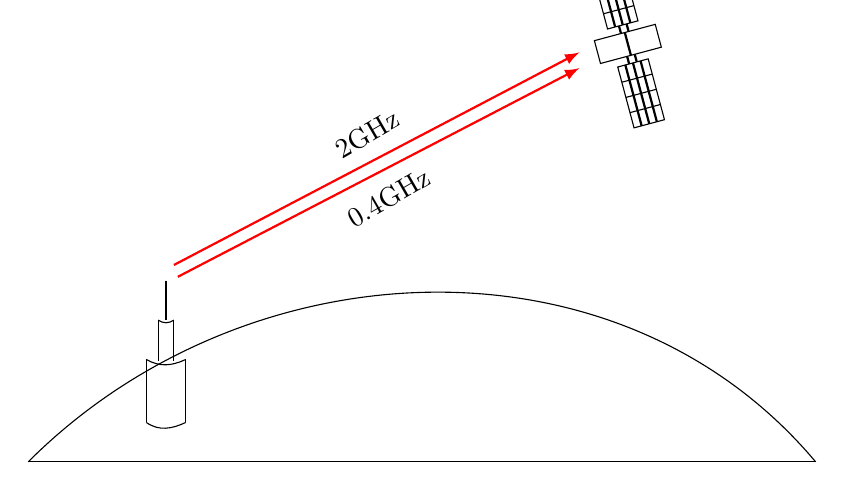
\begin{tikzpicture}
    \coordinate (lend) at (-5, 0);
    \coordinate (rend) at (5, 0);
    \draw (lend) to (rend);
    \draw (lend) to[out=45,in=-230] (rend);

    \coordinate (blb) at (-3.5, 0.5);
    \coordinate (brb) at (-3, 0.5);
    \draw (blb) to[out=-35,in=205] (brb);

    \coordinate (mlb) at (-3.5, 1.3);
    \coordinate (mrb) at (-3, 1.3);
    \draw (mlb) to[out=-30,in=205] (mrb);
    %\draw (mlb) to[out=35,in=-205] (mrb);
    \draw (blb) to (mlb);
    \draw (brb) to (mrb);
    
    \coordinate (tlb) at (-3.35, 1.8);
    \coordinate (trb) at (-3.15, 1.8);
    \draw (tlb) to[out=-35,in=215] (trb);
    \draw (tlb) to (-3.35, 1.28);
    \draw (trb) to (-3.15, 1.28);

    \coordinate (ulb) at (-3.26, 2.3);
    \coordinate (urb) at (-3.24, 2.3);
    \draw (ulb) to (-3.26, 1.8);
    \draw (urb) to (-3.24, 1.8);

    \rotatebox{15}{%
    \draw[] (3.5,4.6) rectangle (4.3,4.3);
    % Up panel
    \draw[thick] (3.9,4.3) to (3.9,4.6);
    \draw[thick] (3.85,4.6) to (3.85,4.7);
    \draw[thick] (3.95,4.6) to (3.95,4.7);
    \draw[] (3.7,5.5) rectangle (4.1,4.7);
    % grid
    \draw[thick] (3.8,4.7) to (3.8, 5.5); 
    \draw[thick] (3.9,4.7) to (3.9, 5.5); 
    \draw[thick] (4.0,4.7) to (4.0, 5.5); 
    \draw[] (3.7,4.9) to (4.1, 4.9);
    \draw[] (3.7,5.1) to (4.1, 5.1);
    \draw[] (3.7,5.3) to (4.1, 5.3);
    % Down panel
    \draw[thick] (3.85,4.3) to (3.85,4.2);
    \draw[thick] (3.95,4.3) to (3.95,4.2);
    \draw[] (3.7,3.4) rectangle (4.1,4.2);
    % grid
    \draw[thick] (3.8,3.4) to (3.8, 4.2); 
    \draw[thick] (3.9,3.4) to (3.9, 4.2); 
    \draw[thick] (4.0,3.4) to (4.0, 4.2); 
    \draw[] (3.7,3.6) to (4.1, 3.6);
    \draw[] (3.7,3.8) to (4.1, 3.8);
    \draw[] (3.7,4.0) to (4.1, 4.0);
    }
    
    \coordinate (satant1) at (2.0,  5.2);
    \coordinate (bcnant1) at (-3.15,2.5);
    \coordinate (satant2) at (2.0,  5.0);
    \coordinate (bcnant2) at (-3.10,2.35);
    \draw[thick,red,-latex] (bcnant1) -- node[above=1mm, align=center, black, rotate=30]{2GHz} (satant1);
    \draw[thick,red,-latex] (bcnant2) -- node[below=1mm, align=center, black, rotate=30]{0.4GHz} (satant2);

\end{tikzpicture}

  \caption{\gls{doris} System Description}
  \label{fig:doris-system-description}
\end{figure}

\subsection{Theoretical Model of Doppler Observations}\label{ssec:doris-obs-theory}
A detailed derivation of the Doppler observation equation, as implemented via the 
\gls{doris} system, can be found in \cite{Lemoine2016}, including a thorough theoretical 
discussion. A brief overview is only given here, with focus on model implementation.

To gain a clear view on the model of the measurements, a rigorous disctinction of 
events must be made; four different events can be identified:
\begin{description}
    \item[beginning of emission] of the 1\textsubscript{st} cycle by the emitter, 
    \(\tau_{e_1}\) in the proper time scale of the emitter and \(t_1\) in the coordinate 
    time
    
    \item[beginning of reception] of the the 1\textsubscript{st} cycle by the receiver, 
    \(\tau_{r_1'}\) in the proper time scale of the receiver and 
    \(t_{1'}\) in the coordinate time

    \item[end of emission] of the N\textsubscript{th} cycle by the emitter, 
    \(\tau_{e_2}\) in the proper time scale of the emitter and \(t_2\) in the coordinate 
    time
    
    \item[end of reception] of the N\textsubscript{th} cycle by the receiver, 
    \(\tau_{r_2'}\) in the proper time scale of the receiver and 
    \(t_{2'}\) in the coordinate time
\end{description}

During the proper time interval $\Delta\tau_{r} = \tau_{r2'} - \tau_{r1'}$, 
the receiver has received the $N_e$ cycles sent by the emitter, with $N_e = f_e \Delta\tau_e$, 
$f_e$ being the proper frequency of the emitter. The receiver is also equipped with
an oscilator and during the proper time interval $\Delta\tau_{r}$ has generated 
a number $N_r = f_r \Delta\tau_r$ of cycles, $f_r$ being the proper frequency of the 
receiver.

The Doppler measurement is the count, by the receiver electronics, of the number 
of cycles of difference between \(N_e\) and \(N_r\):
\begin{equation}
    \begin{split}
    N_{DOP} & = N_e - N_r\\
            & = f_e \Delta\tau_e - f_r \Delta\tau_r
    \end{split}
\end{equation}

\emph{In the RINEX files, this Doppler count is the difference between two phase measurements 
done at different time tags in the proper time-scale of the receiver.}

After a series of assumptions and simplifications, theoretical formula for the 
Doppler count can be written as (\cite{Lemoine2016}):
\begin{equation}
    \begin{split}
        \frac{c}{f_e \Delta\tau_r} N_{DOP} & \approx c \frac{f_e - f_r}{f_e} \\
        & - (1 - \frac{U_e}{c^2} - \frac{{V_e}^2}{2 c^2}) \frac{\rho_2 - \rho_1}{\Delta\tau_r}\\
        & + \frac{1}{c} (U_r - U_e + \frac{{V_r}^2 - {V_e}^2}{2}) \\
        & + \frac{2 \mu}{c^2 \Delta\tau_r} [\ln{(\frac{R_1 + R_{1'} + \rho_1}{R_1 + R_{1'} - \rho_1})} - \ln{(\frac{R_2 + R_{2'} + \rho_2}{R_2 + R_{2'} - \rho_2})}]
    \end{split}
\end{equation}
where
\begin{description}
  \item $c$ is the velocity of light in vacuum,
  \item $f_e$ and $f_r$ are the emitter's and receiver's proper frequencies,
  \item $U_e$ and $U_r$ are the gravitational potential at the emitter and receiver,
  \item $V_e$ and $V_r$ is the velocity of the clock at the emitter and receiver 
    (in the coordinate reference frame),
  \item $\rho _i$ is the curvlinear trajectory (of the photon(s)) at the event $i$,
  \item $R_i$ is the geometric distance between the beacon and the satellite at event $i$
\end{description}

The above equation can be conviniently split into two parts, one containing the ``measured'' 
quantities and one with the ``theoretical'' terms, as 
\begin{subequations}\label{eq:lem12}
  \begin{align}
    v_{measured} & = \frac{c}{f_e} (f_e - f_r -
     \frac{N_{DOP}}{\Delta\tau_r}) + \Delta u_{REL} \label{eq:lem12a} \\
    v_{theo}     &= \frac{\rho_2 - \rho_1}{\Delta\tau_r} (1- \frac{U_e}{c^2} - 
      \frac{{V_e}^2}{2 c^2}) \label{eq:lem12b}
  \end{align}
\end{subequations}
with
\begin{equation}
    \begin{split}
        \Delta v_{REL} &= \frac{1}{c} (U_r - U_e + \frac{{V_r}^2 - {V_e}^2}{2}) \\
        & + \frac{2 \mu}{c^2 \Delta\tau_r} [\ln{(\frac{R_1 + R_{1'} + \rho_1}{R_1 + R_{1'} - \rho_1})} - \ln{(\frac{R_2 + R_{2'} + \rho_2}{R_2 + R_{2'} - \rho_2})}]
    \end{split}
\end{equation}

It is well known that signals transmitted through the Earth's atmosphere are affected by 
it (delayed); let $\Delta v_{IONO}$ and $\Delta v_{TROPO}$, be the propagation corrections of 
the radio electric signal through the ionosphere and troposphere respectively. 

Additionaly, in the actual case (measurements), the nominal frequencies $f_e$ and $f_r$ 
are not the ``true'' ones; hence a relative correction needs to be applied (e.g. for the 
emmiter) $f_{e_T} = f_{e_N} (1 + \frac{\Delta f_e}{f_{e_N}})$, where the subscript $T$ 
denotes the ``True'' frequency and $N$ the nominal one. Thus in \autoref{eq:lem12} the 
terms $f_e$ and $f_r$ need to be substituted by $f_{e_T}$ and $f_{r_T}$ respectively.

$\Delta v_{IONO}$ and $\Delta v_{REL}$, which do not involve adjusted parameters, can be placed 
on the ``measured'' part of \autoref{eq:lem12} and $\Delta v_{TROPO}$ and $\frac{\Delta f_e}{f_{e_N}}$ 
on the ``theoretical'' part. Furthermore, since $\Delta f_e / f_{e_N} \ll 1$ all in 
including $\Delta f_e / f^2_{e_N}$ and $\Delta f^2_e / f^2_{e_N}$ can be safely neglected and 
\autoref{eq:lem12} can be written as:
\begin{subequations}\label{eq:lem13}
    \begin{align}
        v_{measured} & = \frac{c}{f_{e_N}} (f_{e_N} - f_{r_T} -
          \frac{N_{DOP}}{\Delta\tau_r}) + \Delta u_{REL} + 
          \Delta u_{IONO} \label{eq:lem13a} \\
        v_{theo} &= \frac{\rho_2 - \rho_1}{\Delta\tau_r} 
          (1- \frac{U_e}{c^2} - \frac{{V_e}^2}{2 c^2}) + 
          \Delta u_{TROPO} - \frac{c(\frac{N_{DOP}}{\Delta\tau_r} + 
          f_{r_T})}{f_{e_N}} \frac{\Delta f_e}{f_{e_N}} \label{eq:lem13b}
    \end{align}
\end{subequations}
where 
\begin{description}
    \item[\(v_{measured}\)] is the measured relative velocity between the emitter and 
    the receiver between the events 1' and 2', based on the Doppler count \(N_{DOP}\), 
    corrected for the ionospheric and relativistic effects.

    \item[\(v_{theo}\)] is the the theoretical (computed) emitter/receiver relative velocity 
    between the events 1' and 2', corrected for the tropospheric effect and for a solved-for 
    frequency bias \(\frac{\Delta f_e}{f_{e_N}}\) of the emitter. 
    \(f_{r_T} = f_{r_N} (1 + \frac{\Delta f_r}{f_{r_N}})\) 
    is an estimate of the proper frequency of the receiver.

    \item[\(\Delta v_{REL} = \Delta v_{{REL}_c} + \Delta v_{{REL}_r}\)] is the relativistic 
    correction, composed of two parts: the clock correction \(\Delta v_{{REL}_c}\) and the 
    travel correction \(\Delta v_{{REL}_r}\)
    \begin{subequations}\label{eq:lem14}
        \begin{align}
            \Delta v_{{REL}_c} & = \frac{1}{c} 
              (U_r - U_e + \frac{{V_r}^2 - {V_e}^2}{2}) \label{eq:lem14a}\\
            \Delta v_{{REL}_r} & = \frac{2 \mu}{c^2 \Delta\tau_r} \left[ 
              \ln{(\frac{R_1 + R_{1'} + \rho_1}{R_1 + R_{1'} - \rho_1})} - 
              \ln{(\frac{R_2 + R_{2'} + \rho_2}{R_2 + R_{2'} - \rho_2})} \right] \label{eq:lem14b}
        \end{align}
    \end{subequations}
\end{description}

Note that \autoref{eq:lem13} can be further simplified to \autoref{eq:lem17} by 
ommiting small terms (\autoref{ssec:small-terms}).

%\emph{Usually, one frequency offset and one tropospheric zenithal bias are adjusted per pass.}

\subsection{Implementation of the Doppler Observation Model}\label{ssec:obs-model-implementation}

\subsubsection{Small Terms}\label{sssec:small-terms}
In \autoref{eq:lem13}, the smallest terms are \(-U_e / c^2 - {V_e}^2 / 2 c^2\) and 
\(\Delta v_{{REL}_T}\); in the case of \gls{doris} they ammount to \num{11.} and 
\num{6.} \SI{10e-6}{\meter\per\second} respectively (\cite{Lemoine2016}). 
Furthermore, since the emitters are located on the ground, the term 
\(-U_e / c^2 - {V_e}^2 / 2 c^2\) is constant per station. This small 
relativistic offset is absorbed by the adjustment of \(\Delta f_e / f_{e_N}\). 
So it is possibly to furher simplify \autoref{eq:lem13} to:
\begin{subequations}\label{eq:lem17}
    \begin{align}
        v_{measured} & = \frac{c}{f_{e_N}} (f_{e_N} - f_{r_T} -
          \frac{N_{DOP}}{\Delta\tau_r}) + 
          \Delta u_{{REL}_C} + \Delta u_{IONO} \label{eq:lem17a}\\
        v_{theo} &= \frac{\rho_2 - \rho_1}{\Delta\tau_r} + \Delta u_{TROPO} - 
          \frac{c(\frac{N_{DOP}}{\Delta\tau_r} + f_{r_T})}{f_{e_N}} 
          \frac{\Delta f_e}{f_{e_N}} \label{eq:lem17b}
    \end{align}
\end{subequations}

\subsubsection{Correction of Aberration}\label{sssec:doris-aberration}
In \autoref{eq:lem13} (or \autoref{eq:lem17}), $\rho _i$ is the geometrical distance 
between the emitter at time $t_i$ and the receiver at time $t_{i'}$ (with $i=1,2$). 
The measurements are made by the receiver electronics, hence the instance $t_i$ is 
actually unknown. In order to compute accurately $t_i$ and thus the position of 
the emitter at this istant in time, a \emph{correction of aberration} (\cite{Lemoine2016}) 
has to be performed. This correction can be evaluated in an iterative manner: an 
approximate value of of the emitter-receiver distance $\rho ^{*} _i$ is first computed, 
by evaluating the position of the beacon at time $t_{i'}$. Subsequently, $t_i$ can be 
found via $t_i = t_{i'} - \rho ^{*} _i / c$. In practice, one iteration is enough.

\subsubsection{Geopotential}\label{sssec:doris-geopotential}
For a station on the geoid, the potential at the level of the station is the sum 
of the gravitational potential and the centrifugal potential due to the Earth's 
rotation: $U_{GEO} = U_e + \frac{{V_e}^2}{2}$, which is a constant. For a station 
not located on the geoid, the quantity $U_e + \frac{{V_e}^2}{2}$ will only depend 
on the height of the beacon above the geoid.

For the computation of the gravitational potential for \gls{leo} satellites, 
the pottential $U_r$ cannot be restricted to the central term only ($GM_{\Earth} / r$) and
the Earth's oblateness ($J_2$) effect should also be considered (\cite{Larson2007}). 
Hece, the equation used reads (\cite{Lemoine2016})
\begin{equation}\label{eq:lem18}
  U_r = 
    -\frac{GM_{\Earth}}{r} \left( 
      1 - 
      \left( \frac{R_{\Earth}}{r} \right) ^2 
      J_2 \frac{3 sin^2(\phi) - 1}{2} 
    \right)
\end{equation}
or in cartesian coordiates (\cite{Larson2007})
\begin{equation}
  U_r = -\frac{GM_{\Earth}}{r} \left( 1- \left(\frac{R_{\Earth}}{r}\right)^2 
    J_2 \frac{3 z^2 - r^2}{2r^2} \right)
\end{equation}
with $R_{\Earth}$ the equatorial radious of the earth, $r$ radial 
distance of the satellite (to the Earth's center), $\phi$ latitude of the 
satellite and $J_2 = 1.0826359 \dot 10^{-3}$ in the zero-tide system (\cite{iers2010}).

\subsubsection{True Proper Frequency of the Receiver}\label{sssec:true-proprtfrequency-of-the-receiver}
For the term $f_{r_T}$ that appears in \autoref{eq:lem13}, we need an estimate of 
$\Delta f_{r} / f_{r_N}$. This estimate can be obtained in one of the following ways 
\cite{Lemoine2016}:
\begin{enumerate}
    \item via the field ``F'' recorded for every single measurement in the \gls{doris} 
      RINEX file (see \autoref{ssec:relative-frequency-offset}); not that this estimation 
      is not very smooth, as noticed by \cite{Gao2015} and it is advisable, before 
      using it in \autoref{eq:lem13}, to perform a linear (or polynomial) regression of 
      these estimates over one or a few days.
    \item It can also be obtained from a polynomial regression
      over the frequency offsets estimated during the passes
      over the master beacons
    \item It can finally be estimated by the users themselves as a
      by-product of their re-computation of the timetagging polynomial (see \cite{Mercier2010})
\end{enumerate}

\subsubsection{Nominal Receiver \& Emitter Frequencies}\label{ssec:nominal-frequencies}
In the observation equation model \autoref{eq:lem13} we distinguish between 
\emph{nominal} and \emph{true} receiver/emitter frequencies, to account for 
the fact that in ``real world'' these two are not actually equal.

\paragraph{Emitter (Beacon) Nominal Frequencies, $f_{e_N}$}\label{par:beacon-nominal-frequencies}
RINEX file headers, contain values of the \emph{station frequency shift 
factor} $k$ for each of the beacons involved (\cite{DORISRNX3}, Sec. 6.16). 
These are used to compute the ``nominal'' frequencies of the beacon/emitter 
(usually, this shift factor is just $0$, but it can be an integer 
$k \neq 0$). The frequencies are computed as (\cite{DORISRNX3}, Sec. 6.16):
\begin{equation}
  \begin{aligned}
    L_{2GHz}   &= 543 \cdot F_0 \left( \frac{3}{4} + \frac{87\cdot k}{5 \cdot 2^{26}} \right) \\
    L_{400MHz} &= 107 \cdot F_0 \left( \frac{3}{4} + \frac{87\cdot k}{5 \cdot 2^{26}} \right) 
    \label{eq:nominal-freq}
  \end{aligned}
\end{equation}
where $F_0 = 5e6 \text{ Hz}$ the \gls{uso} frequency. These value, are the ones 
labelled as $f_{e_N}$ in \autoref{eq:lem13}.

The \emph{true proper frequency} of the emitter $f_{e_T}$, can be computed 
from:
\begin{equation}
  f_{e_T} = f_{e_N} \cdot \left( 1 + \frac{\Delta f_e}{f_{e_N}} \right)
\end{equation}
but the quantity $\Delta f_e / f_{e_N}$ is not know a-priori and has to be 
estimated during the processing.

The quantity $\Delta f_e / f_{e_N}$  can be estimated either as a constant term (bias), 
or using a linear model (bias ad drift). In the latter case (followed in this Thesis), 
the model can be written as:
\begin{equation}
  \frac{\Delta f_e}{f_{e_N}}\at{\tau=\tau _i} = \alpha + \beta \cdot \delta \tau
\end{equation}
%with an a-priori value of 0 and no process noise. 
For the estimation, we need the partials of the observation equation \autoref{eq:lem13b} 
w.r.t. the $\alpha$ and $\beta$ parameters, which are:
\begin{equation}
  \begin{aligned}
  \frac{\partial v_{theo}}{\partial \alpha} &= 
    \frac{c(\frac{N_{DOP}}{\Delta\tau_r} + f_{r_T})}{f_{e_N}} \\
  \frac{\partial v_{theo}}{\partial \beta} &= 
    \frac{c(\frac{N_{DOP}}{\Delta\tau_r} + f_{r_T})}{f_{e_N}} \cdot \delta \tau
  \end{aligned}
\end{equation}

\paragraph{Receiver True Proper Frequency $f_{r_T}$}\label{par:receiver-true-proper-frequency}
In \autoref{eq:lem13}, $f_{r_T}$ is the \emph{true proper frequency of 
the receiver} with nominal value 
\begin{equation}\label{eq:frt-gen}
  f_{r_T} = f_{r_N} \cdot \left( 1 + \frac{\Delta f_r}{f_{r_N}} \right)
\end{equation}
where $f_{r_N}$ is the ``nominal'' frequency value.

In practice the value $\Delta f_r / f_{r_N}$, called the \emph{relative 
frequency offset} of the receiver, is given in the RINEX files for each epoch 
(under the observable tagged \texttt{F}). Note that these values are scaled to 
$10^{-11}$ (\cite{DORISRNX3}, Sec. 6.11), so that for a given epoch $t_i$, the 
true frequency is
\begin{equation}\label{eq:frt-rinex}
  f_{r_T}\at{t=t_i} = f_{r_N} \cdot \left( 1 + F_{t_i} \cdot 10^{-11} \right)
\end{equation}
where $F_{t_i}$ is the relative frequency offset value recovered from the RINEX 
file.

\iffalse
\fi

\subsection{Ionospheric Correction}\label{ssec:iono-correction}
The basic observation equation \autoref{eq:lem13}, is formed for the \SI{2}{\GHz} 
carrier. For each measurement, the ionospheric path delay has to be corrected for, 
by computing a correction (in cycles) as (\cite{Lemoine2016}, Sec. 2.5.7):
\begin{equation}
  \delta_{ION} [\SI{2}{\GHz}\text{ cycles}] = 
    \frac{L_{\SI{2}{\GHz}} - \sqrt{\gamma} \cdot L_{\SI{400}{\MHz}}}{\gamma - 1}
  \label{eq:iono-delay-cycles}
\end{equation}
which is added to the \SI{2}{\GHz} measurement at time $t=t_i$ (obtained by the 
RINEX file). Thus, the corrected observation is:
\begin{equation}\label{eq:l2if}
  L_{\SI{2}{\GHz},IF} [\SI{2}{\GHz}\text{ cycles}] = 
    L_{\SI{2}{\GHz}} + \delta_{ION}
\end{equation}

Note that after applying \autoref{eq:l2if}, the measurement is refered to the ``Iono-Free'' 
geometrical endpoints of the signal path (and not the \SI{2}{\GHz} endpoints). 
This means that the respective {phase center corrections (i.e. \gls{pco} and \gls{pcv})
both at the satellite and at the beacon have to be applied.
